\documentclass{beamer}

% Setting Presentation Fonts
\usepackage{fontspec}
\setmainfont[Ligatures=TeX,BoldFont={*-Bold}]{Times-New-Roman}
\setsansfont[Ligatures=TeX,BoldFont={*-Bold}]{Times-New-Roman}
\setmonofont{Courier-New}

% For Images
\usepackage{tikz}

% New CTU fonts
\newfontfamily\technikaregular{Technika-Regular.ttf}
\newfontfamily\technikaitalic{Technika-Italic.ttf}
% Additional Technika Fonts are Available from https://campuscvut.sharepoint.com/sites/inforek-ma (after login)

% Defining Title Page Inputs

% Title
\title{\uppercase{A Brief Report on Permanent Magnet Assisted Synchronous Reluctance Motors}}

% Subtitle
%\subtitle{\uppercase{{Very long name of a presentation which is currently build in a LaTeX
%}}} % download italic technika when available

% Author
\author{Petr Zakopal}

% Supervisor
\newcommand{\SupervisorTitle}{XP14DES}
\newcommand{\SupervisorName}{}

% Opponent
\newcommand{\OpponentTitle}{}
\newcommand{\OpponentName}{}

% End of Defining Title Page Inputs

% Extra texts in FootLine and FrameTitle
\newcommand{\FootLineLeft}{\uppercase{Department of Electric Drives and Traction}}
\newcommand{\FrameTitleRight}{\uppercase{Faculty of Electrical Engineering in Prague}}

\newcommand{\cvutlogo}{
\includegraphics[scale=0.2]{src/misc/symbol_cvut_plna_verze.pdf}}


% Defining frame title based on a technika font and color
\newcommand{\techbluetitle}[1]{
    \begin{center} 
            {\fontsize{16pt}{16pt}\technikaregular {\color{ctublue}#1}}
    \end{center} 
}

% Selecting which theme to use
\usetheme{k13114}

\begin{document}

% \addtobeamertemplate{frametitle}{}{%
% \begin{tikzpicture}[remember picture,overlay]
%   \node[anchor=north west,yshift=5pt,xshift=-5pt] at (current page.north west) {\cvutlogo};
% \end{tikzpicture}}

% \addtobeamertemplate{footline}{}{%
% \begin{tikzpicture}[remember picture,overlay]
%   \node[anchor=south east,yshift=-5pt,xshift=3.5pt] at (current page.south east) {\cvutlogo};
% \end{tikzpicture}}


	\frame {
		\titlepage
	}
	\frame {
		\frametitle{Table of contents}
        %\vspace*{-2cm}
        %\techbluetitle{Structure of the report}
         {\fontsize{16pt}{16pt}\technikaregular {\color{ctublue}Structure of the report}}
        %\vspace*{1.8cm}
        \begin{itemize}
            \item Introduction            \item Design
            \item Control
            \item Comparison to other machines
            \item Recent research interest   
        \end{itemize}
	}
	\frame{
		\frametitle{Introduction}

        {\fontsize{14pt}{14pt}\technikaregular {\color{ctublue}PMSynRelM}}\par
        \vspace*{0.5cm}
        {\fontsize{14pt}{14pt}\technikaregular {\color{ctugrey}actively used in automotive and traction aplications}}\par
        \vspace*{0.5cm}
        {\fontsize{14pt}{14pt}\technikaregular {\color{ctugrey}control strategies based on known principles}}\par
        \vspace*{0.5cm}
        {\fontsize{14pt}{14pt}\technikaregular {\color{ctugrey}may use relatively simple mathematical model for control}}\par
        \vspace*{0.5cm}
        {\fontsize{14pt}{14pt}\technikaregular {\color{ctugrey}PMSynRelM}}
	}
	\frame{
		\frametitle{Introduction}

        {\fontsize{14pt}{14pt}\technikaregular {\color{ctugrey}PMSynRelM}}\par
        \vspace*{0.5cm}
        {\fontsize{14pt}{14pt}\technikaregular {\color{ctublue}actively used in automotive and traction aplications}}\par
        \vspace*{0.5cm}
        {\fontsize{14pt}{14pt}\technikaregular {\color{ctugrey}control strategies based on known principles}}\par
        \vspace*{0.5cm}
        {\fontsize{14pt}{14pt}\technikaregular {\color{ctugrey}may use relatively simple mathematical model for control}}\par
        \vspace*{0.5cm}
        {\fontsize{14pt}{14pt}\technikaregular {\color{ctugrey}PMSynRelM}}
	}
	\frame{
		\frametitle{Introduction}

        {\fontsize{14pt}{14pt}\technikaregular {\color{ctugrey}PMSynRelM}}\par
        \vspace*{0.5cm}
        {\fontsize{14pt}{14pt}\technikaregular {\color{ctugrey}actively used in automotive and traction aplications}}\par
        \vspace*{0.5cm}
        {\fontsize{14pt}{14pt}\technikaregular {\color{ctublue}control strategies based on known principles}}\par
        \vspace*{0.5cm}
        {\fontsize{14pt}{14pt}\technikaregular {\color{ctugrey}may use relatively simple mathematical model for control}}\par
        \vspace*{0.5cm}
        {\fontsize{14pt}{14pt}\technikaregular {\color{ctugrey}PMSynRelM}}
	}
	\frame{
		\frametitle{Introduction}

        {\fontsize{14pt}{14pt}\technikaregular {\color{ctugrey}PMSynRelM}}\par
        \vspace*{0.5cm}
        {\fontsize{14pt}{14pt}\technikaregular {\color{ctugrey}actively used in automotive and traction aplications}}\par
        \vspace*{0.5cm}
        {\fontsize{14pt}{14pt}\technikaregular {\color{ctugrey}control strategies based on known principles}}\par
        \vspace*{0.5cm}
        {\fontsize{14pt}{14pt}\technikaregular {\color{ctublue}may use relatively simple mathematical model for control}}\par
        \vspace*{0.5cm}
        {\fontsize{14pt}{14pt}\technikaregular {\color{ctugrey}PMSynRelM}}
	}
	\frame{
		\frametitle{Introduction}

        {\fontsize{14pt}{14pt}\technikaregular {\color{ctugrey}PMSynRelM}}\par
        \vspace*{0.5cm}
        {\fontsize{14pt}{14pt}\technikaregular {\color{ctugrey}actively used in automotive and traction aplications}}\par
        \vspace*{0.5cm}
        {\fontsize{14pt}{14pt}\technikaregular {\color{ctugrey}control strategies based on known principles}}\par
        \vspace*{0.5cm}
        {\fontsize{14pt}{14pt}\technikaregular {\color{ctugrey}may use relatively simple mathematical model for control}}\par
        \vspace*{0.5cm}
        {\fontsize{14pt}{14pt}\technikaregular {\color{ctublue}PMSynRelM}}
	}
	\frame{
	    \frametitle{Design}
        \techbluetitle{Stator}
	}
	\frame{
	    \frametitle{Stator Design}
        \begin{minipage}[t]{0.30\textwidth}
            \begin{itemize}
                \item \textcolor{ctured}{Delta} winding
                \item \textcolor{ctublue}{Star} winding
                \item \textcolor{ctublue}{Star}-\textcolor{ctured}{Delta} hybrid winding
            \end{itemize}
        \end{minipage}%
        \hfill
        \begin{minipage}[t]{0.68\textwidth}
            \begin{figure}[H]
                \centering
                    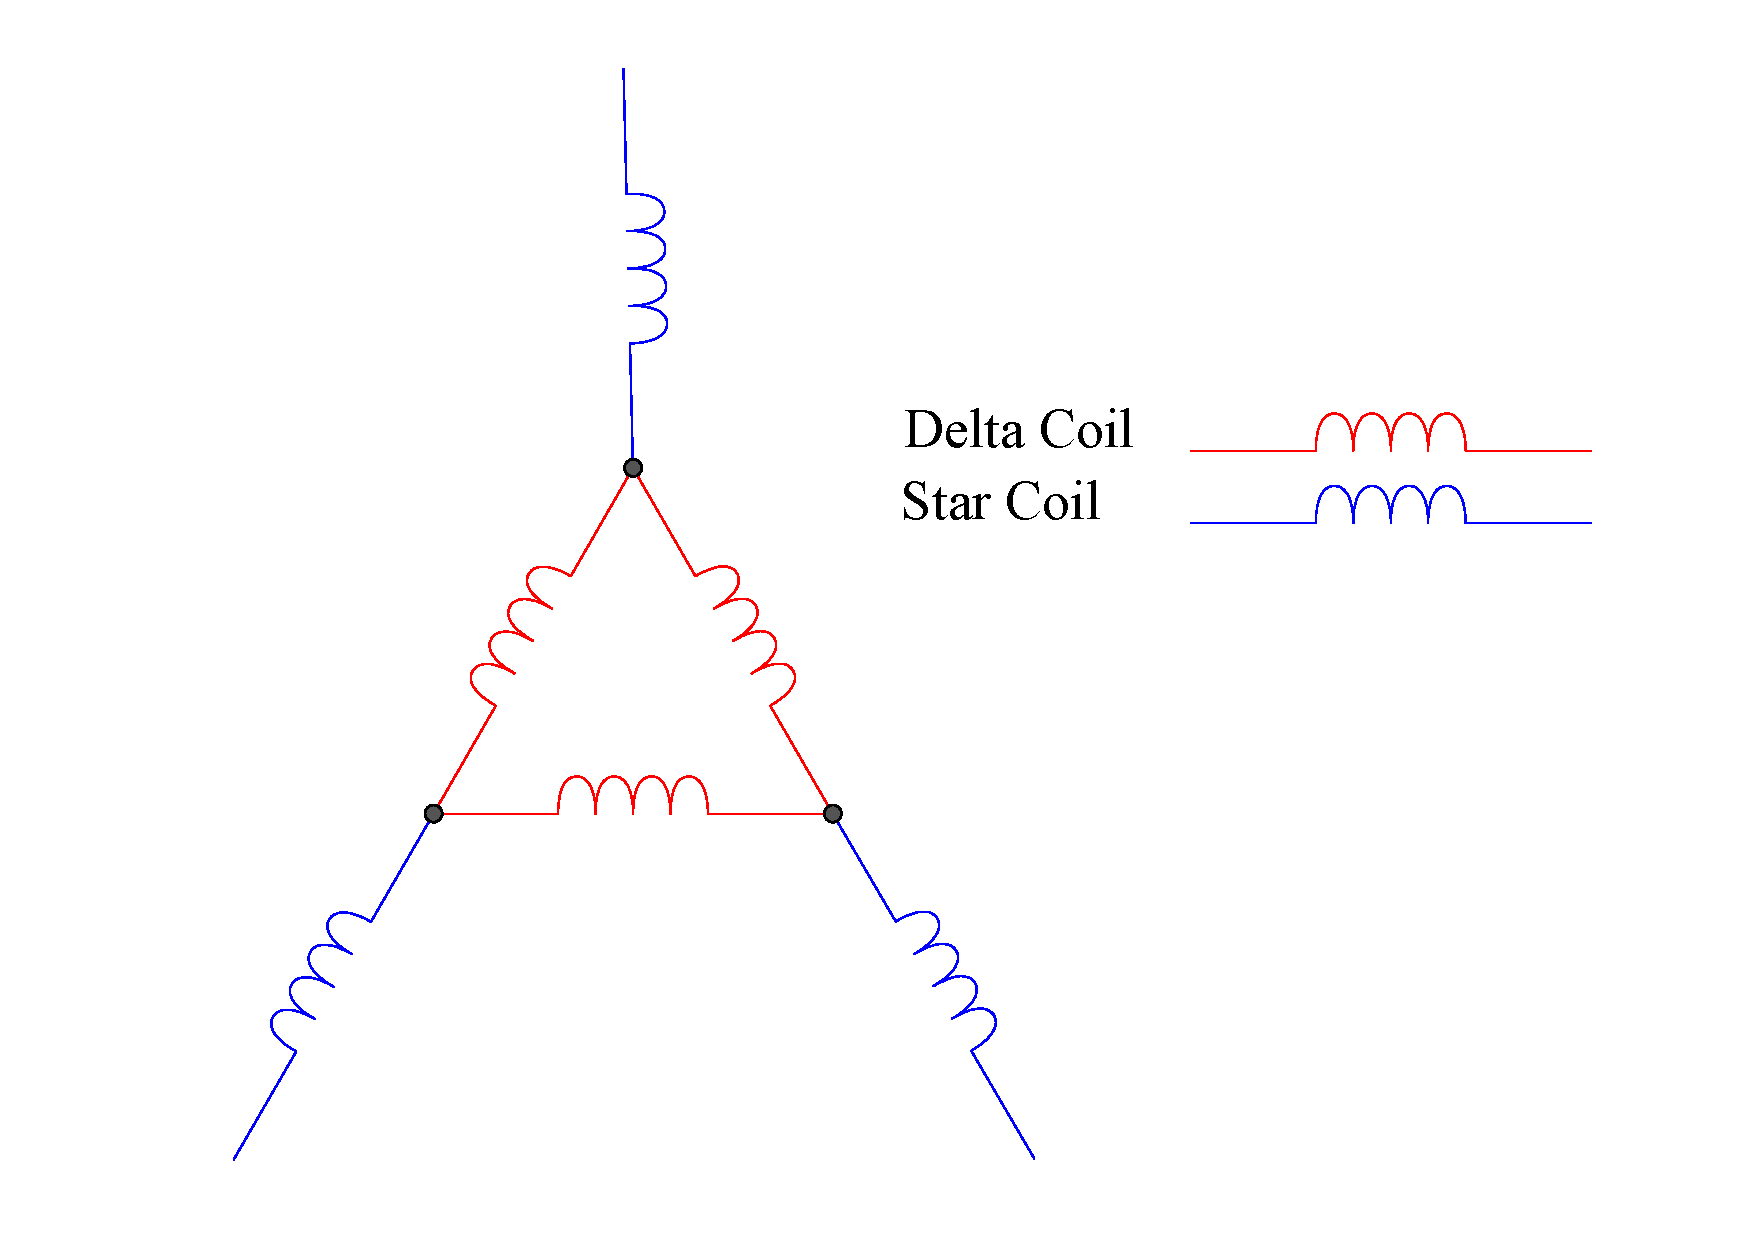
\includegraphics[width=0.75\textwidth]{./../tex/src/pdf/hybrid-star-delta-wiring.pdf} 
            \end{figure}
        \end{minipage}

	}
	\frame{
	    \frametitle{Design}
        \techbluetitle{Rotor}
	}

\end{document}
